\documentclass[letterpaper,11pt,twoside]{article}
\usepackage[utf8]{inputenc}
\usepackage{amsmath,amsfonts,amssymb,amsthm,latexsym}
\usepackage[spanish,es-noshorthands]{babel}
\usepackage[T1]{fontenc}
\usepackage{lmodern}
\usepackage{graphicx,hyperref}
\usepackage{tikz,pgf}
\usepackage{multicol}
\usepackage{fancyhdr}
\usepackage[height=9.5in,width=7in]{geometry}
\usepackage{fancyhdr}
\pagestyle{fancy}
\fancyhead[LE]{
\includegraphics[height=12pt]{Images/logo-colegio.png} Geometría $6^{\circ}$}
\fancyhead[RE]{}
\fancyhead[RO]{\textit{Germ\'an Avenda\~no Ram\'irez, Lic. U.D., M.Sc. U.N.}}
\fancyhead[LO]{}

\author{Germ\'an Avenda\~no Ram\'irez, Lic. U.D., M.Sc. U.N.}
\title{\begin{minipage}{.2\textwidth}

\includegraphics[height=1.75cm]{Images/logo-colegio.png}\end{minipage}
\begin{minipage}{.55\textwidth}
\begin{center}
Taller 06, La medida es cosa seria\\
Geometría $6^{\circ}$
\end{center}
\end{minipage}\hfill
\begin{minipage}{.2\textwidth}

\includegraphics[height=1.75cm]{Images/logo-sed.png} 
\end{minipage}}
\date{}
\thispagestyle{plain}
\begin{document}
\maketitle
Nombre: \hrulefill Curso: \underline{\hspace*{44pt}} Fecha: \underline{\hspace*{2.5cm}}
\begin{multicols}{2}
 \section*{Explora tus conocimientos}
 Para hacer unas reformas de carpintería en su casa, Rosario compró los siguientes materiales:
\begin{itemize}
\item 10 listones de 2 m
\item 21 listones de 75 cm
\item 50 listones de 15 Dm
\item 100 pequeños listones de 1 dm
\item 1 rollo de alambre de 10 Dm
\end{itemize}
Observe que no es lo mismo dm que Dm, en el primer caso se representan decímetros y en el segundo Decámetros.
\begin{itemize}
\item[a.] ¿Cuántos centímetros de listón compró en total?
\item[b.] Si devolvió la mitad de los listones pequeños, y la tercera parte de los grandes, ¿cuántos metros utilizó en las reformas?
\item[c.] ¿Cuántos metros de alambre empleó?
\end{itemize}
\section*{¿Qué est\'{a} cerca y qu\'{e} est\'{a} lejos}
Intuitivamente conocemos lo que es longitud o largo. En la práctica, lo que realmente medimos es la distancia o separación entre dos puntos, y dependiendo de la unidad de medida elegida, podemos decidir si uno de los puntos está cerca o lejos del otro.

En esta guía estudiarás las unidades pactadas universalmente para medir, no solamente longitudes; también las que se usan para medir superficies y el tiempo.
\section*{Lo que s\'{e}}
En grupos de 3 personas desarrollar en el cuaderno de cada uno las siguientes actividades:
\begin{itemize}
\item Fijen dos puntos diferentes y alejados uno del otro, en un
espacio abierto del colegio, coloquen un objeto en cada punto
elegido. Luego, cada uno de los integrantes del grupo debe
contar la cantidad pasos que separan esos dos puntos.
\item Anoten los resultados en sus cuadernos, en una tabla como la siguiente.
\begin{center}
\begin{tabular}{|l|p{1.4cm}|p{1.4cm}|p{1.4cm}|}
\hline 
Estudiante &  &  &  \\ 
\hline 
Número de pasos &  &  &  \\ 
\hline 
\end{tabular} 
\end{center}
\begin{itemize}
\item Comparen los datos registrados en la tabla. ¿Los resultados son iguales o diferentes?
\item ¿Por qué creen que se presentan diferencias, si las hay?
\item ¿Cómo se podrían evitar estas diferencias?
\end{itemize}
\item Midan algunos objetos con la palma de la mano.

Por ejemplo, una mesa del salón. Comiencen por uno de los
extremos y apoyen sus manos una a continuación de la otra a
lo largo de un lado de la mesa. Cuenten.
Cada uno de los integrantes del grupo debe determinar
cuántas veces cabe su mano en el lado de la mesa y completar
la siguiente frase en su cuaderno.

El lado de la mesa mide \underline{\hspace*{24pt}} manos.

Con el mismo procedimiento midan el alto de la mesa: desde
el piso hasta la tabla donde se apoyan los útiles escolares y
completen el siguiente enunciado.

La mesa mide \underline{\hspace*{24pt}} manos de alto.
\begin{itemize}
\item ¿Es práctico medir el ancho y el largo del salón de clases con las manos? ¿Y para distancias largas, como el recorrido de su casa a la escuela?
\end{itemize}
\item Piensen elementos que sirvan para medir, por ejemplo: la
regla. ¿Les parece necesario tener una medida universal para
medir? Expliquen su respuesta.
\end{itemize}
\section*{Aprendo algo nuevo}
Si se mide sin ningún instrumento, se hace una estimación
de la medida.

Y si se eligen distintas unidades para una misma cantidad, se
obtienen medidas diferentes, lo cual impide comparar cantidades de una determinada magnitud y dificulta las operaciones.
Con el propósito de evitar los inconvenientes de elegir diferentes unidades para hacer mediciones, en casi todos los
países del mundo se ha adoptado el Sistema Internacional de Medidas (\textbf{SI}) que es la forma actual del \textbf{Sistema Métrico Decimal}.

Las unidades fundamentales del Sistema Internacional de Medidas son las siguientes:
\begin{center}
\begin{tabular}{|l|c|c|}
\hline 
\qquad \textbf{Magnitudes} & \textbf{Unidad} & \textbf{Símbolo} \\ 
\hline 
Longitud & Metro & m \\ 
\hline 
Masa & Kilogramo & Kg \\ 
\hline 
Tiempo & Segundo & s \\ 
\hline 
Corriente eléctrica & Ampere & A \\ 
\hline 
Temperatura & Kelvin & K \\ 
\hline 
Intensidad luminosa & Candela & cd \\ 
\hline 
Cantidad de sustancia & Mol & mol \\ 
\hline 
\end{tabular} 
\end{center}
Otras unidades del SI, algunas de las cuales estudiarás en
cursos posteriores, son:
\begin{center}
\begin{tabular}{|l|c|c|}
\hline 
\qquad \textbf{Magnitud} & \textbf{Unidad} & \textbf{Símbolo} \\ 
\hline 
Superficie & Metro cuadrado & $m^{2}$ \\ 
\hline 
Volumen & Metro cúbico & $m^{3}$ \\ 
\hline 
Capacidad & Litro & L \\ 
\hline 
\end{tabular} 
\end{center}
\begin{itemize}
\item Indiquen la unidad correspondiente en el Sistema Internacional de Medidas para cada magnitud.
\begin{tabbing}
\hspace{3cm}\=\kill
Longitud \> Masa \\ 
Capacidad \> Superficie 
\end{tabbing}
\item Dibujen un segmento y mídanlo con una regla.
\begin{itemize}
\item ¿Qué magnitud midieron?
\item ¿Cuánto mide el segmento que dibujaron?
\item ¿Qué unidad utilizaron?
\end{itemize}
\end{itemize}
El \textbf{metro} (m) es la unidad fundamental de \textbf{longitud}.
\begin{itemize}
\item Pidan ayuda a su profesor y tracen en el piso una recta de longitud 1 m. ¿Cuántos pasos caben en 1 m? ¿Cuántos palmos?
\end{itemize}
Para medir longitudes menores que un metro se utilizan unidades más pequeñas denominadas \textbf{submúltiplos} del metro.
\begin{center}
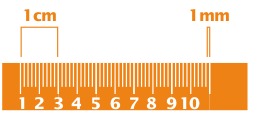
\includegraphics[scale=.9]{Images/regla.png} 
\end{center}
Cada una de las diez partes iguales en que se divide un metro se llama \textbf{decímetro}. 1 m = 10 dm

Cada una de las diez partes iguales en que se divide un decímetro se llama \textbf{centímetro}. 1 m = 10 dm = 100 m

Cada una de las diez partes iguales en que se divide un centímetro se llama \textbf{milímetro}. 1 m = 10 dm = 100 cm = 1 000 mm
\begin{itemize}
\item Propongan algunos ejemplos de longitudes para las cuales sea conveniente utilizar el decímetro, el centímetro y el milímetro, como unidades de medida.
\end{itemize}
Para medir longitudes mayores que el metro se utilizan unidades más grandes llamadas \textbf{múltiplos del metro}.

Un \textbf{decámetro} equivale a diez metros. 1 Dm = 10 m

Un \textbf{hectómetro} es igual a cien metros. 1 hm = 10 Dm = 100 m

Un \textbf{kilómetro} equivale a mil metros. 1 km = 10 hm = 100 Dm = 1\,000 m
\begin{itemize}
\item Se puede estimar una longitud de 1 m fácilmente
\begin{itemize}
\item Estimen cuántos decámetros hay en el ancho y el largo del colegio.
\item Nombren distancias a su alrededor, que midan 1 hm y 1 km.
\item Estimen la distancia que cada uno debe recorrer para ir de la casa al colegio.
\end{itemize}
\end{itemize}
\end{multicols}
\end{document}
